%The background should set the project into context by motivating the subject matter and relating it to existing published work. The background will include a critical evaluation of the existing literature in the area in which your project work is based and should lead the reader to understand how your work is motivated by and related to existing work.
\chapter{Background}
This chapter aims to introduce some concepts surrounding our problem domain, which aim to help the reader understand and easily follow the subsequent, more technical chapters. It also presents a review of the related work that has been done in this area. The sections below in this Chapter look at some of the key aspects and problems that arise. I then conclude by providing a summary of the alternatives that are presented.

%number of alternative methods for solving our problem.

%Explain Curtailments (short turning) - reasons for this are: delays, planned roadworks or events, insufficient layover, improve overall realiability of the service fill gaps, prevent breaches - drivers hours regulation
%Bus bunching 
\section{London Bus Network}
The London bus network is one of the most advanced and renowned in the world. It runs 24 hours and it is extensive and frequent. Every route in the network is tendered to different bus company operator \cite{busTendering}. Each of these bus operator companies is then responsible for abiding to the contracts with TFL. This means that they (the different bus companies) are responsible to ensure that the services they are operating run according to the timetable as per the respective contract. There are two main types of schedules that are being used:
\begin{itemize}
	\item Fixed - a bus stop need to be served at specific predefined times (e.g. 1:00pm, 1:20pm, 2:00pm etc.).
	\item Headway based - this means that buses should serve bus stops at regular intervals (e.g. a stop needs to be visited by a bus every 5 minutes).
\end{itemize}

However, under different circumstances some delays occurring on a given route are beyond the control of the individual bus operator companies. A simple example could be a burst water/gas pipe on a street used by a bus route or any other incident (even terrorist attacks \cite{centreComm}) and even simply a severe congestion. In situations like this, bus operators have no authority or power to respond or overcome such problems on their own. This is where CentreComm comes into place to respond and deal with these issues. In situations like this the bus drivers or operators would need to alert and ask CentreComm to intervene. The emergency command and control room at TFL can do so by, for example implementing a short/long term diversions or curtailments (short turning) on/for some of the buses on the affected routes. They (CentreComm) can also seek assistance from London Traffic Control Centre\footnote{\url{http://www.tfl.gov.uk/corporate/about-tfl/what-we-do/roads}} or even the Police under given circumstances.

Buses in the network can be classified by multiple factors however, for the purpose of this report, the main distinction we need to consider, apart from fixed and headway based schedules are \textbf{high} and \textbf{low} frequency bus routes \cite{busTendering}. High frequency routes are those where 5 or more buses attend a given stop per hour, whereas low frequency routes are those that have a stop being visited by 4 or less buses an hour.

%there are 5 or more buses per hour attending a given bus stop. Low frequency routes are those that have 4 or less buses at a stop.
%These operators agree with TFL that the routes they are operating would be served either according to a predefined fixed schedule (e.g. a bus stop need to be served at 1pm, 3pm etc.)or on a headway (e.g. a bus stop need to be served every 5 minutes).
\section{CentreComm}
CentreComm is TFL's emergency command and control room, responsible for all public buses in London. It has been in operation for more than 30 years \cite{centreComm} and it employs a dedicated team of professionals who work 24 hours a day, 364 days in the year. They are dealing with more than a 1000 calls on a daily basis. The majority of these calls come from bus drivers or bus company operators regarding problems and incidents happening within the bus network. CentreComm staff implement planned long and short term changes in the bus network in response to different events taking place in the capital (including the 2012 Olympics). They are also responsible for reacting in real time to any unexpected and unpredicted changes and disruptions, maintaining the smooth, reliable and sage operation of London's busy bus network.

London bus network consists of around 680 bus routes operated by more than 8000 buses \cite{glads}. Each of these buses is equipped with state of the art iBus system to help monitor and manage this enormous fleet. CentreComm's way of operation has been transformed beyond recognition since it has first opened. It started more than 30 years ago \cite{centreComm} when it consisted of a couple of operators equipped with two way radios, pen and papers. Today CentreComm operators make use of numerous monitor screens, each displaying interactive maps (showing the location of each bus in the network) and CCTV cameras, in real-time. However, there is still a lot of room for automation and improvement in their way of operation in order to effectively and efficiently deal with the growing bus network and its demands.

%CentreComm is not responsible for the fleet management as mentioned above. The emergency control and command room comes into place when there are planned or unplanned events affecting the bus network which need to be taken care of. They are responsible in assisting the bus drivers and bus company operators to manage their schedules when there are events which are beyond their control.
%CentreComm is not responsible for the fleet management as this is contracted to the bus operators which are responsible for maintaining reliable service according to agreed contracts. The emergency control room comes in place when there are planned or unplanned events which disrupt the transport network. They are also responsible for helping the bus operators once they cannot maintain the service they are responsible for due to traffic congestion or other issues which are beyond their control. However currently CentreComm relies on the bus drivers and bus operators for letting them know of such cases as they do not have a system which to signal them about these issues. All the information they need is there and they have access to it however they do not have the resources to manually monitor each of the 8000+ buses.
\section{iBus AVL}
Automatic vehicle location (AVL) systems provide vehicle tracking, usually in real time. Most often this is achieved by the integration of Global Positioning System (GPS), wireless communications (e.g. SMS, GPRS) and geographic information system (GIS) \cite{riter1977automatic}. AVL systems employ wireless communications for the transmission of the GPS coordinates and other data of the vehicle as it moves in the transport network. Once received by the a central server or computer, this information allows the GIS software to map the location of the vehicle and it also enables further analysis to be performed based on the data.
 
%Automatic vehicle location systems make use of the Global Positioning System (GPS) to enable the remote (using the internet) tracking of the locations of the vehicles in a given fleet. This system combines a number of technologies including GPS, cellular communications and more with the goal of improving and cutting the cost of fleet management. 

All of London buses operating on the TFL bus network have been equipped with state of the art and award wining \cite{ibusAward} AVL system named iBus \cite{ibus}. This system has opened a range of new applications that could be built on top of it, using the information that is made available. The iBus system consist of a number of computer and communication systems, sensors and transmitters as described in \cite{Hounsell201276} and \cite{eps354267}. One of the key components of the system is the on-board unit (OBU) which is mounted on each of the buses in the TFL bus fleet and consists of a computational unit connected to sensors and GPS transmitters (see figure~\ref{fig:iBusOverview} below taken from \cite{Hounsell201276}).
\begin{figure}[ht]
	\makebox[\textwidth][c]{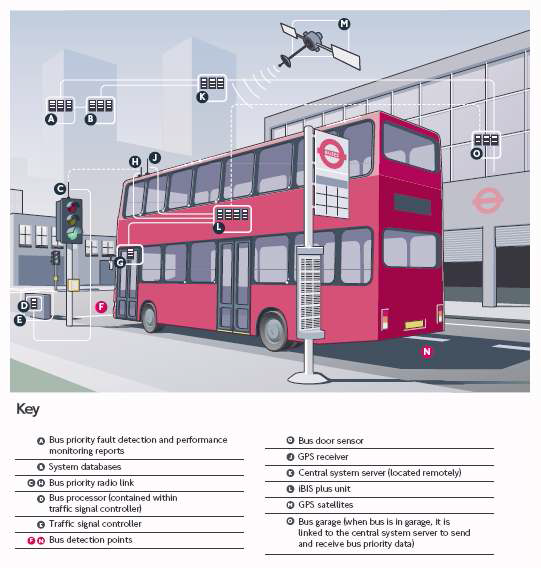
\includegraphics[width=1\textwidth]{Figures/iBus.png}}
	\caption{Overview of iBus System \cite{Hounsell201276}}
	\label{fig:iBusOverview}
\end{figure}
The OBU is responsible for a number of tasks including a regular (approximately every 30 seconds) transmission of the bus location. This information is currently used by the different bus operators for fleet management, as well as by CentreComm for real-time monitoring of the buses and their locations. There have been a number of other applications and systems that have been implemented and put in to use as a result of the data that is generated by the iBus AVL. Some examples include Countdown (real-time passenger information), improved bus priority at traffic signals and more \cite{Hounsell201276}. This has led to improved and more affordable transport service.

CentreComm operators have access to an online GIS system showing each bus location in the network on a map in real time. This system also allows them to see whether a given bus is behind, ahead or on time according to its schedule. However, this does not show or alert the control room staff if a bus or a route is disrupted. Control room staff can also see when was a given bus expected to arrive at a given bus stop and when it actually arrived. Again, this is only per individual bus and there are no automatic alerts set, in case a given route or stop is experiencing delays. Currently the work-flow is such that on-duty CentreComm staff needs to go and analyse all this information manually (once bus drivers or bus company operator have contacted/alerted the control room) in order to figure out if there is a problem and how severe it actually is. This is a very inefficient, tedious and error-prone process. Here is where this project comes into place to address the lack of preprocessed information and automated alerts.

\section{Related Work}
The literature is full of research towards accurately predicting bus arrival times with various computational models being used \cite{altinkaya2013urban}. Predicting bus arrival is complex as many factors need to be considered such as, bus dwell time at stops, general congestion and others \cite{jeong2005prediction}. This is also closely related to the issues of bus prioritisations for which we can find numerous examples in the literature. Some examples of work done towards bus prioritisation at traffic signals and junctions can be found in \cite{eps52676} and \cite{clarke2007}. However, these are not directly related to our problem domain and thus are not discussed further in this report. This is because we are not interested to know when is the next bus due to arrive at a stop or should we give priority to a bus at traffic signal. We want to know if buses experience increased travel time, because of which they get delayed travelling through some parts of the network. 
 
%The literature is abundant of research on addressing the issues of bus prioritisation at traffic signals and junctions \cite{eps52676} and \cite{clarke2007}, but this is not directly related to our problem domain and thus is not discussed further in this report.
 
%This however is not what this project is about as we are not interested to know when is the next bus due to arrive at stop, but we want to know if buses get delayed travelling through some parts of the network. 

The main problem posed by this project of detecting disruptions in the bus network can be also translated to short term traffic congestion detection and/or travel time calculation. This is valid as we are not interested in individual bus delays. Some examples of such single instances of bus disruptions are: customer incident on board of a single bus, technical fault with this bus or other issue(s) which are affecting a single vehicle rather than the entire route or network. We are interested into finding routes/sections in the network which are delayed/disrupted and this is beyond the control of individual bus operators. Most often such problems are due to some sort of congestion or road closures/repairs. However, road problems are in most cases linked with increased traffic congestions as roads are used by other vehicles as well. In order to address this problem we have focussed our attention towards work which relates to calculating the bus travel times or gives short-term traffic congestion predictions in a given transport network.

The literature contains plenty of work done toward detecting and calculating travel times in non-urban environment. This includes approaches based on AVL probe data and automatic vehicle identification (AVI), as well as induction loops \cite{Vlahogianni20143}. There is also plenty of research done towards traffic congestion detection based on AVL probe data \cite{Vlahogianni20143}. However, there are significant challenges due to the nature of the urban environment itself. Densely populated areas are influenced by many factors which can be affecting the general traffic flow. Another problem posed by urban environments is the irregularity of the AVL data transmission because of, for example weak or lost signal at times (e.g. due to high buildings) or even the presence of some noise which reduces the accuracy of the transmitted location. 

There is however, little research to my knowledge, which focusses on the issues of detecting and short-term forecasting traffic congestion/disruptions in arterial urban environment  \cite{Vlahogianni20143} \cite{5625144}. From the tables shown in figures ~\ref{fig:Vlahogianni201431} to ~\ref{fig:Vlahogianni201434} in Appendix A taken from \cite{Vlahogianni20143} we can easily see that most of what has been done has focussed on motorways and also has employed data from static detector points (e.g automatic vehicle identification). Only in recent years we can see that more attention has been given to the use of GPS and AVL data. This is probably due to increased popularity and usage of these technologies.

%As it can be seen from the tables in figures ~\ref{fig:Vlahogianni201431} to ~\ref{fig:Vlahogianni201434} shown in Appendix A taken from \cite{Vlahogianni20143}.

%For this reason in order to address our problem domain however we are not interested specifically in the general congestion as this could for example not affect the operation of the TFL bus fleet directly. A simple reason for this could be because there are significant amount of street which have a designated bus lanes which are prohibited for use by the general traffic. However there are studies showing that even under such circumstances there is a correlation between the general traffic flow and the performance of the buses in the same network [REFERENCE]. For our project we are interested however only in detecting the disrupted routes (sections of routes) and the severity of the disruption in the TFL bus network. We are interested in monitoring and detecting delays that are occurring in the network which would be classified, beyond the control of individual bus operator, by CentreComm.

%The literature review that has been undertaken as part of this project has showed that there are multiple approaches that could be undertaken to solve the problem posed by this project. There could be found different classifications of the models for predicting bus travel time\cite{surveyAIApplications}. According to \cite{urbanBusArrivalTimeCompModels} we could classify them into four computational models:
%\begin{itemize}
%	\item Based on historical data
%	\item Statistical 
%	\item Kalman Filtering 
%	\item Machine Learning
%\end{itemize}
%We could also add hybrid model which takes a combinational from the above [REFERENCE].

%The approaches and research that we have examined show us that the the main types of models that have been used for traffic forecasting according to \cite{youKim} can be categorised as follows:
In the literature various approaches to measure and predict travel time can be found. These models are categorised in four type groups according to \cite{youKim} as follows:
\begin{itemize}
	\item Statistical models - this type of models employ statistical tools and methods for analysis and forecasting. Some models of this type include:
	\begin{itemize}
		\item Historical
		\item Time Series
		\item Nonparametric regression
		\item Hybrid
	\end{itemize}
	
	\item Computer Simulations - main models of this type are traffic simulations. They allow simulation of the traffic flow in a network resembling the characteristic of moving vehicles. Main advantage of these models is that they allow for the simulation of different scenarios. The main drawback however, is that they require traffic flow prediction information in advance \cite{smith1997traffic}. Due to the optimisation nature of these approaches, usually high performance computers are employed (i.e. in \cite{junchaya1992advanced} they make use of parallel computing).
	
	\item Mathematical Optimisation - this include dynamic traffic assignment (DTA) models. A good review of dynamic traffic assignment and simulation models can be found in \cite{mahmassani1991review}.

	\item Artificial Intelligence (AI) - neural networks are an example of AI approach. They have received a lot of attention in terms of transportation systems applications. Some examples include traffic signal control, traffic flow modelling and transportation planning \cite{gilmore1995neural,Dougherty199721,smith1997traffic}.
\end{itemize}
The advantages and disadvantages of the listed types and models are summarised in table showed in figure~\ref{fig:modelsProsCons} below.

\begin{figure}[ht]
	\makebox[\textwidth][c]{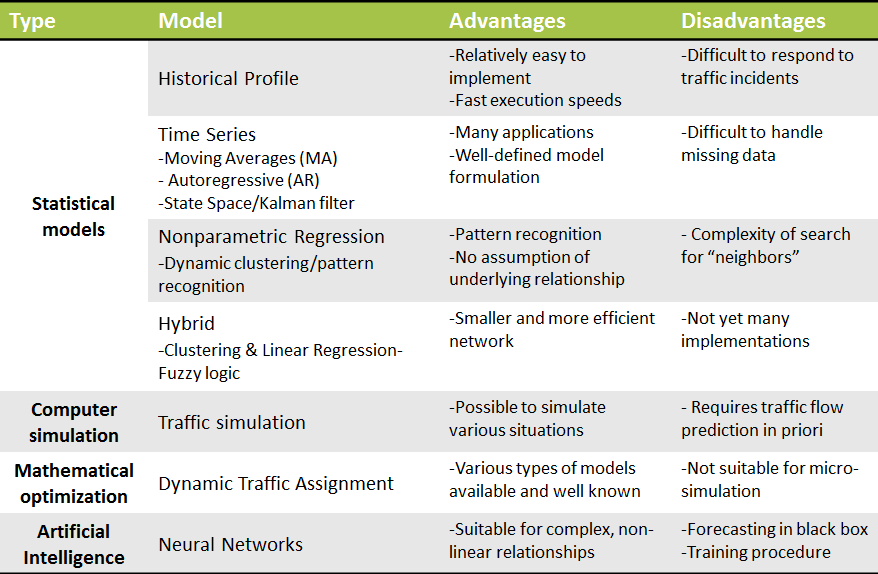
\includegraphics[width=1\textwidth]{Figures/modelsProsCons.png}}
	\caption{Traffic forecasting types and models \cite{youKim}}
	\label{fig:modelsProsCons}
\end{figure}

From the above mentioned, the most widely used and well defined are the statistical models. From them the historical approaches are relatively easy for implementation and have fast execution speed, but have difficulty with dealing with incidents. Time series models have many applications and are well formulated. Because of these reasons and also the nature of the data that has been made available (detailed description of which can be found in Chapter 5) for this project, we will focus our attention on time series analysis for the rest of this report.

\section{Time Series}
Time series is a sequence of data readings taken during successive time intervals \cite{shumway2010time}. This could be a continuous recording of readings or a set of discrete readings. In the context of our project we have the continuous process of bus readings (generated by the AVL system) being transmitted which generate a discrete set of observations. This results in a data set of measurement values which consists of the actual values with some noise. Time series data contains four main components (illustrated in figure~\ref{fig:timeSeriesDataComponents})\cite{brockwell2002introduction}:
\begin{itemize}
	\item \textbf{Trend} - this is the long term pattern that the given time series data follows. The trend can have positive or negative value depending on whether the data exhibits an increase or decrease respectively in the long term pattern. Time series data with no trend (it does not show nether increase or decrease) is said to be stationary.
	\item \textbf{Cyclical} - this is when we can see that the data show up and down movement around a given trend is referred to as cyclical pattern. Main characteristic of the cycle is its duration which can depend on the type of measurement.
	\item \textbf{Seasonal} - seasonality occurs when the time series exhibits regular repetetive fluctuations. For instance, temperatures peaks during summer months (in the northern hemisphere) and drop during winter months.
	\item \textbf{Irregular} - also known as the error component. These are random increases or decreases for a specific time period.
\end{itemize}

\begin{figure}[ht]
	\makebox[\textwidth][c]{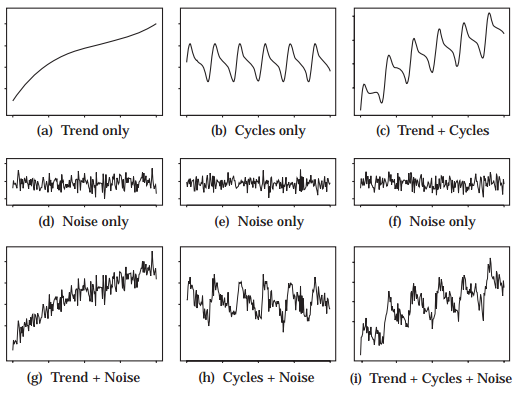
\includegraphics[width=1\textwidth]{Figures/timeSeriesDataComponents.png}}
	\caption{Time series data components examples taken from \cite{wildchance}}%taken from https://www.stat.auckland.ac.nz/~wild/ChanceEnc/Ch14.pdf
	\label{fig:timeSeriesDataComponents}
\end{figure}

Analysis of time series data could be performed in order to extract and calculate some meaningful statistics from the data \cite{shumway2010time}. This could also result in producing a forecast of the data of interest for the next (future/unobserved) period of time based on the past observations. In order to highlight trends and make predictions, we need to employ time series analysis techniques. Below I have presented some of the available techniques that could be employed when analysing time series data. This however, is not an exhaustive review of all available methods and models as I have tried to keep the discussion relevant to this project.

%Time series analysis is performed on time series data in order to extract some meaningful statistics from the data. In addition to the time series analysis time series forecasting could also be performed to come up with a prediction for the next period in time based on what has been observed in the past. In our problem this would mean having a number of bus readings we could analyse them and come up with prediction of what would be state in the next point in time. There also different smoothing techniques which would remove random abnormal fluctuation (e.g. an incident with a single bus).In the below sections we look at a number of different approaches to analysing and forecasting the next state of the network from the available data in real-time (we update our forecast whenever more data becomes available).

\subsection{Moving Averages}
One technique commonly used in time series analysis is moving averages which represent a form of smoothing. Smoothing means to dampen the effect of noise and irregularities in the original time series. Moving average, also called rolling or running average is a statistical calculation method. It helps to analyse data series by calculating a series of averages of subsets of the data. Moving averages are commonly used in time series data analysis when the data is fairly stable and does not have significant trend, cyclical or seasonal effects. It can be used in order to smooth out a time series data with the aim of highlighting or estimating the underlying trend of the data. The other main usage is as a forecasting method, again for time series. The main strength of these methods is that they are easy to understand. Moving averages are often used as the building block for more complex time series analysis. Below we present some of the main types of moving averages that are used in practice. \cite{brockwell2009time,shumway2010time}

%It is universal analysis technique. It is type of mathematical convolution \cite{shumway2010time}.It can also be referred to as rolling or moving mean and it acts like a filter.
\subsubsection{Simple Moving Average}
Simple moving average (SMA) is calculated by adding all the observations for a given period of time and dividing this sum by the number of observations. This is popular statistical technique which is mainly used to calculate the trend direction. The simple average is only useful for estimating the next forecast when the data does not contain any trends. Each observation is weighted equally. If we consider shorter period window (meaning we only consider less observation e.g. only the last 5 or 10) for our averages they would react quicker to changes. While if we work with bigger period windows the averages would have greater lag. The equation for calculating SMA is given below in equation~\ref{sma}. In this $n$ is the size of the window (e.g. the number of reading we are considering) and $Value(i)$ is the actual value of observation $i$. 

\begin{equation}\label{sma}
	SMA = \frac{\sum_{0\le i\le n}\textrm{Value(i)}}{n}
\end{equation}

In the table on figure~\ref{fig:smaTable} we can see sample time series data with window size $n$ equal to $3$. The graph in figure~\ref{fig:smaGraph} shows the plotted actual observation values and the SMA calculated predictions.

\begin{figure}[ht]
	\makebox[\textwidth][c]{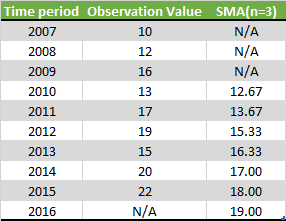
\includegraphics[]{Figures/smaTable.png}}
	\caption{}
	\label{fig:smaTable}
\end{figure}

\begin{figure}[ht]
	\makebox[\textwidth][c]{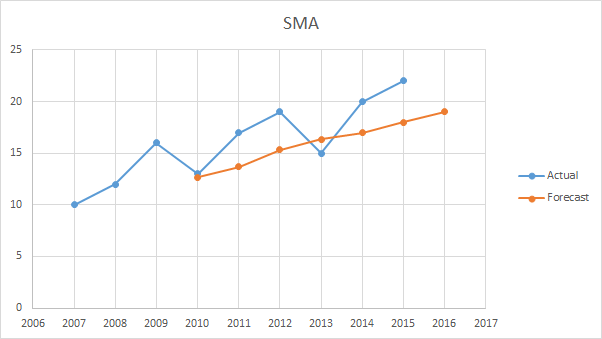
\includegraphics[]{Figures/smaGraph.png}}
	\caption{}
	\label{fig:smaGraph}
\end{figure}

Another form of SMA is centered moving average (CMA). Both are very similiar in terms that they use the same method for calculating the average value, but they differ in that the CMA calculates an average of $n$ periods' data and associates it with the midpoint of the periods. An example can be seen in figures~\ref{fig:cmaTable} and \ref{fig:cmaGraph}.

\begin{figure}[ht]
	\makebox[\textwidth][c]{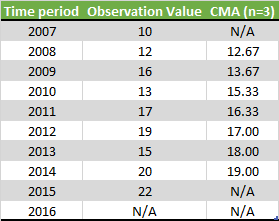
\includegraphics[]{Figures/cmaTable.png}}
	\caption{}
	\label{fig:cmaTable}
\end{figure}

\begin{figure}[ht]
	\makebox[\textwidth][c]{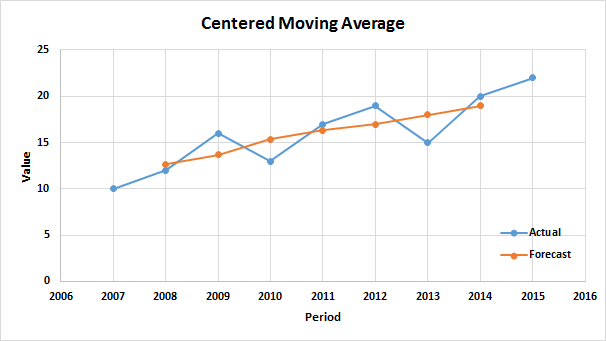
\includegraphics[]{Figures/cmaGraph.png}}
	\caption{}
	\label{fig:cmaGraph}
\end{figure}

\FloatBarrier
\subsubsection{Weighted Moving Average}
The problem with the simple moving average is that it weighs all data points equally, meaning that both older and newer data would have the same effect on the average. This however, is not the case when using weighted moving average (WMA). In WMA model each data point would be weighted differently according to the period of time when the observation was made. For example, if we consider a $n$ period moving average we can calculate the weight for the value taken in period $i$ where $0\le i\le n$ by the following formula: \[\textrm{Weight(i)} = \frac{2i}{n(n+1)}\] This would mean that recent data has bigger impact on the result. However it should be noted that the weighting formula given is only an example as it is the most natural and widely used weigthing scheme for WMA. It is possible to use different weighting formula, one such alternative could be: \[\textrm{Weight(i)} = \frac{2^i}{\sum_{0\le x\le n}2^x}\] this would result in putting more weight on more recent data (e.g. older data is having less effect). The general equation for calculating WMA is given below as equation~\ref{wma}, where $n$ is the number of observations (the size of the window).

\begin{equation}\label{wma}
WMA = \frac{\sum_{0\le i\le n}(\textrm{Weight(i)}\textrm{Value(i)})}{\sum_{0\le i\le n}Weight(i)}
\end{equation}

An example of the application of WMA is shown in the table in figure~\ref{fig:wmaTable}. The forecast is plotted against the actual values and is shown in the graph in figure~\ref{fig:wmaGraph}

\begin{figure}[ht]
	\makebox[\textwidth][c]{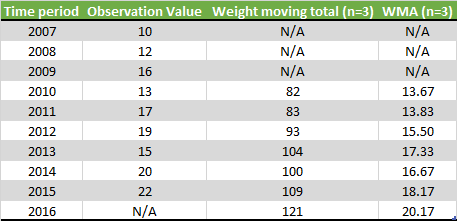
\includegraphics[]{Figures/wmaTable.png}}
	\caption{}
	\label{fig:wmaTable}
\end{figure}

\begin{figure}[ht]
	\makebox[\textwidth][c]{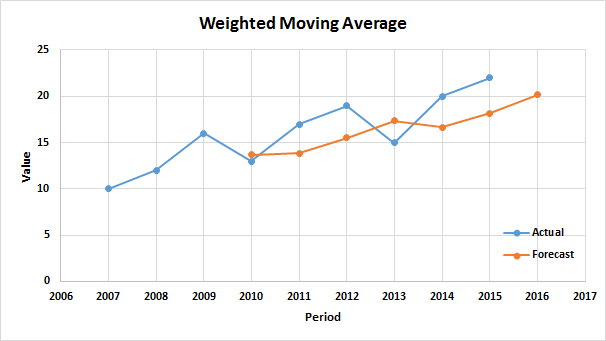
\includegraphics[]{Figures/wmaGraph.png}}
	\caption{}
	\label{fig:wmaGraph}
\end{figure}

\FloatBarrier
\subsubsection{Exponentially Weighted Moving Average}
Exponential smoothing was first suggested by Robert Goodell Brown \cite{FOR3980040103}. Exponentially weighted moving average (EWMA) or also called exponential smoothing or simply exponential moving average (EMA) is very similar to WMA. The main difference is that in order to calculate it, we do not need to keep all the data, but we could only store the latest value and the previous forecast only. Exponential moving average weights the data points exponentially which means that the oldest data would have minimalistic effect on the result. There exist a few exponential smoothing techniques including single, double and triple exponential moving average [REFERENCE]. Equations 2.3 and 2.4 give the simplest way for calculating single exponential smoothing. In this equation $\alpha$ is called the smoothing factor and it is usually a value between $0$ and $1$. The closer $\alpha$ is to $0$, the greater smoothing effect it has. This however makes it less responsive to recent changes thus produces greater lag. Values of $\alpha$ that are near to $1$ have less smoothing effect, but are very reactive to recent changes in the data. 

\begin{align}\label{ema}
EMA_1 = Value_1 \\
\textrm{for } t > 1\textrm{, }EMA_t = \alpha Value_t + (1-\alpha) EMA_{t-1}
\end{align}

Example of the application of EMA with different values of $\alpha$ ($0.2$ and $0.8$) is shown in figures~\ref{fig:emaTable} and~\ref{fig:emaGraph}. From this simple example it can be clearly seen the effect the value of $\alpha$ has on the output value. From the graph (figure~\ref{fig:emaGraph}) it can be seen that the smaller $\alpha$ value of $0.2$ has greater smoothing effect, but greater lag. The bigger value of this constant increases the reactivity to recent changes, but produces less smoothed line.
\begin{figure}[ht]
	\makebox[\textwidth][c]{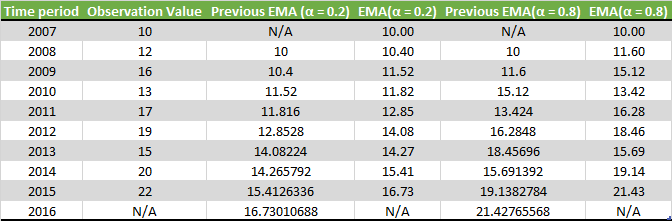
\includegraphics[]{Figures/emaTable.png}}
	\caption{}
	\label{fig:emaTable}
\end{figure}

\begin{figure}[ht]
	\makebox[\textwidth][c]{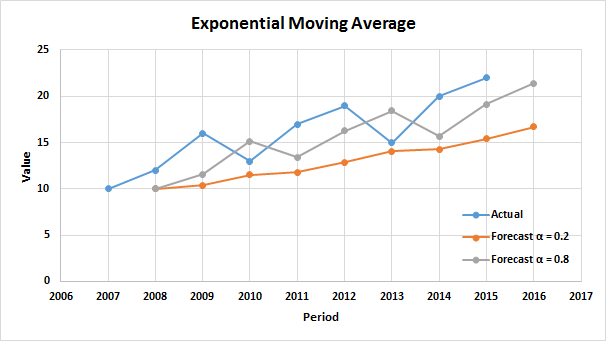
\includegraphics[]{Figures/emaGraph.png}}
	\caption{}
	\label{fig:emaGraph}
\end{figure}
%Exponential Smoothing for Predicting Demand. Cambridge, Massachusetts: Arthur D. Little Inc. p. 15.] and then expanded by Charles C. Holt in 1957.[Holt, Charles C. (1957). "Forecasting Trends and Seasonal by Exponentially Weighted Averages". Office of Naval Research Memorandum 52. reprinted in Holt, Charles C. (January–March 2004). "Forecasting Trends and Seasonal by Exponentially Weighted Averages". International Journal of Forecasting 20 (1): 5–10. doi:10.1016]
\FloatBarrier
\subsubsection{Summary}
If we compare the presented moving average methods (SMA, CMA, WMA and EMA) we can clearly see that the SMA and CMA offer the most smoothing. However, this comes with the trade-off of an increased lag (e.g. it takes longer to reflect recent changes). 

The weighted moving average performance is influenced by the choice of window size, as well as the choice of weights. There is no single rule what weights one should use and most often this is based on intuition and simulations in order to get optimal results.

As we have seen in the given examples, the exponential moving average performance depends heavily on the chosen values for the $\alpha$ constant. EMA offers the advantage of not having to keep all data point values in memory for the periods of our window. Whereas all the other presented techniques require us to specify a widow size for our moving average and also to have the data for these periods available in memory. The choice of window size for the SMA, CMA and WMA has direct impact on the sensitivity (speed of reaction) of the method to changes. Increased size of the window results in less reactive moving average and increase in the opposite.

If a trend indication with better smoothing and little reaction for shorter movements is required, then the simple average should produce the best results. However if smoothing is desired where you can still see shorter movements, then it is better to use either WMA or EMA. Using either of those techniques, requires us to make some choices regarding what parameters (window size and weight for WMA and value of $\alpha$ for EMA) to use in order to obtain best results.

%will react faster to changes and sits closer to the actual readings, however it might overreach at times. 
%The weighted moving follows the movement even more closely than the exponential moving average. Determining which one to use depends on the objective. 

\subsection{Peak Detection}
Peaks and valleys represent significant events where the graph changes from increasing to decreasing behaviour and vice versa (decreasing to increasing). In the domain of our project we are mostly concerned with peak detection as we are not interested to know if buses are gaining time (e.g. are going ahead of schedule). Mathematically viewed peaks and valleys represent local maxima and local minima respectively \cite{simon1994mathematics}.

Detection and analysis of peaks (spikes) and valleys in time series is important in many applications (e.g signal processing, bioinformatics, medicine and many more) \cite{ventzas2011peak}. Peaks and valleys usually represent either significant events or errors in time series data. In our domain we are mostly interested in detecting high sudden changes in the traffic congestion conditions (e.g along route/sections in the bus network). In figure~\ref{fig:peakExampleGraph} we can see an example of such peak (highlighted in red) we would be interested to detect.

\begin{figure}[ht]
	\makebox[\textwidth][c]{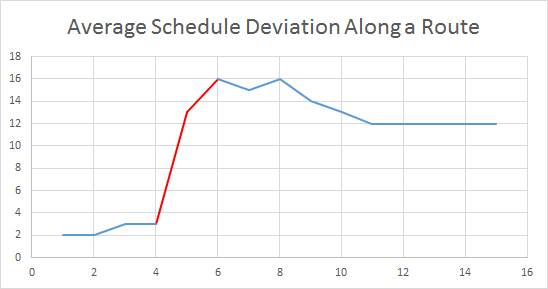
\includegraphics[]{Figures/peakExampleGraph.png}}
	\caption{X-axis shows us the sections along the route and the Y-axis represents the schedule deviation in minutes}
	\label{fig:peakExampleGraph}
\end{figure}

Peaks could be easily identified by visualising the data as in the above example. However, to be relevant and useful in real application this process should be automated. Various peak searching algorithms are studied and presented in \cite{ventzas2011peak}.

%In the literature has many examples of peak detection application one such for example is \cite{simplePeakDetection} used for spike detection in microarray data (anther example could be found in \cite{Azami2014491}).

%We do not go into details of any particular algorithms here because of the time constraints of this project (a study peak detection algorithms could be found in \cite{ventzas2011peak}).

\FloatBarrier
%\section{Other}
%However it is worth to note that spike detection and analysis could be used to classify events that are detected. A simple example could be to distinguish if given detected congestion/disruption is incident related (e.g. sudden) or it is general traffic jam (e.g. rush hour).
%[MOVE THIS TO CONCLUSION AS DIRECTION FOR FUTURE WOKR] - check this http://www.cs.technion.ac.il/users/wwwb/cgi-bin/tr-get.cgi/2012/CS/CS-2012-06.pdf
%Other approaches that could be used include Kalman filtering \cite{kalmanFiltering} \cite{Guo201450}, Markov Chains \cite{Qi201495} \cite{Ramezani20121576}, Machine learning \cite{herring2010real}, Bayesian networks \cite{Wang201479}. 

%In this report we do not go into further details of these alternative  as the aim of the project is to fully understand the requirements of the CentreComm and propose a prototype which to serve as a proof of concept.
%Markov chain is a stochastic process that transitions from one state to another using some state space. It is characterised by the property of having no memory. This means that the next state depends only on the current state and not on the preceding sequence of state transitions. This is called a Markov property.
%Markov chains are usually used in modelling many practical problems. They are also effective in modelling time series. In this paper, we apply the Markov chains model to analyse and predict the time series. Some series can be expressed by a first-order discrete-time Markov chain and others must be expressed by a higher order Markov chain model. Numerical examples are given. The results show that the performance and effectiveness of the Markov chain model to predict the time series is very well.[TAKEN FROM - Application of Markov Chains to Analyze and Predict the Time Series]

\section{Summary}
In this chapter I have aimed to provide the reader with broad view of the background of our problem and its domain. Detailed overview of the operations, technologies and work flows used by TFL's bus command and control centre has been provided. This has led to detailed review and discussion of the related work found in the literature. The chapter concluded with discussion on some of the available time series analysis methods that can be used in our project. The exact approach taken and any implementation specifics are described in detail in Chapter 5, along with presentation and discussion of the data that has been provided by TFL for this project.